
%%%%
%%%%  FIGURE 
%%%%
\begin{figure}[h!]
   \vbox{
     \hbox{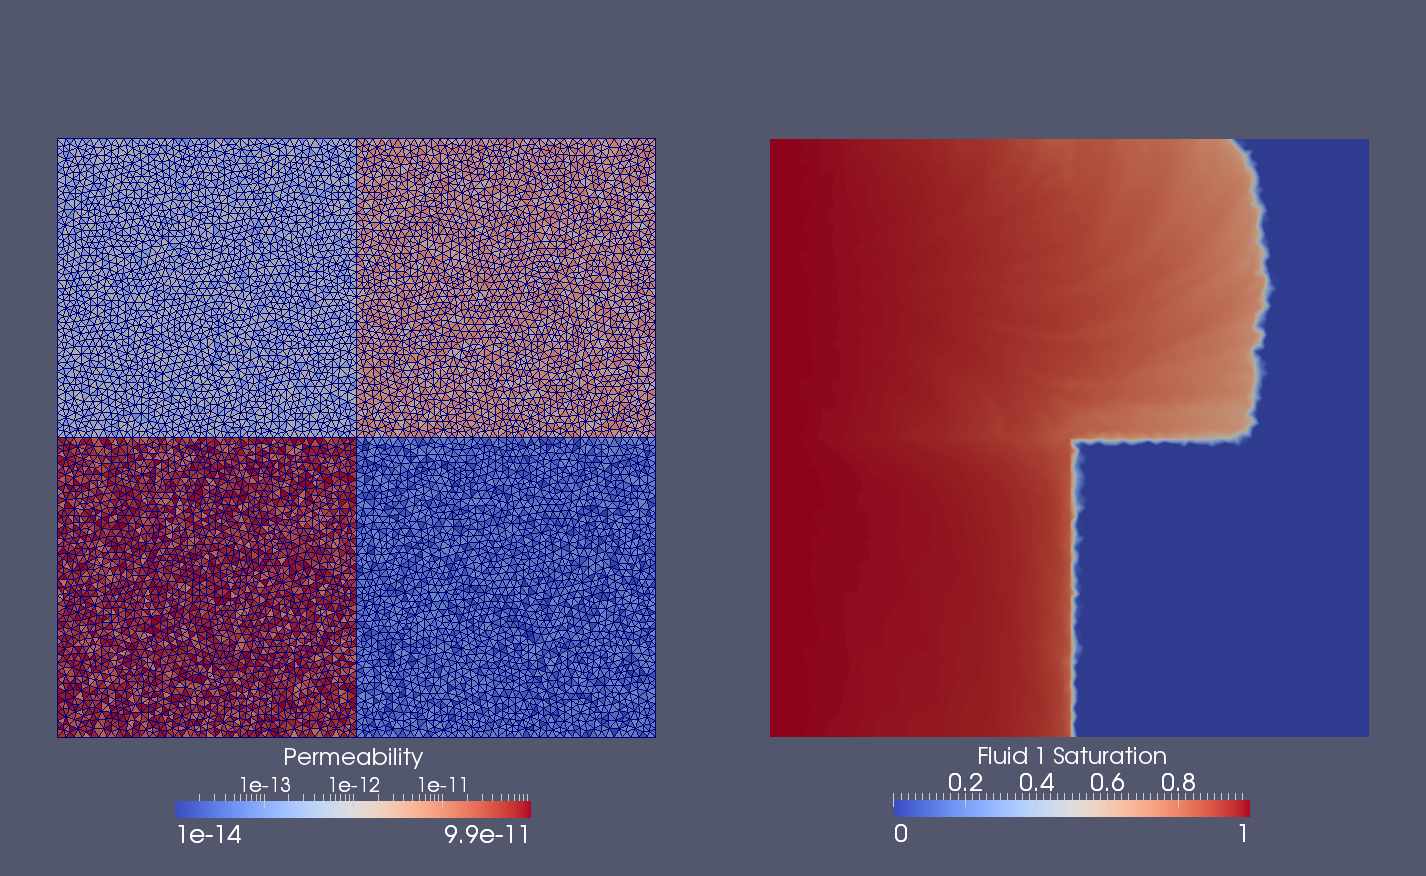
\includegraphics[width=\columnwidth,clip]{./Pics/PermField_Saturation.png}}
     \hbox{\hspace{4cm}(a)\hspace{7.8cm}(b)}}
        \caption{(a) Permeability distribution and (b) phase saturation showing preferential flow pathways.}
        \label{fig:PermField_Saturation}  
\end{figure}
\clearpage

%%%%
%%%%  FIGURE
%%%%
\begin{landscape}
\begin{figure}[ht] 
\vbox{\vspace{-1cm}
\hbox{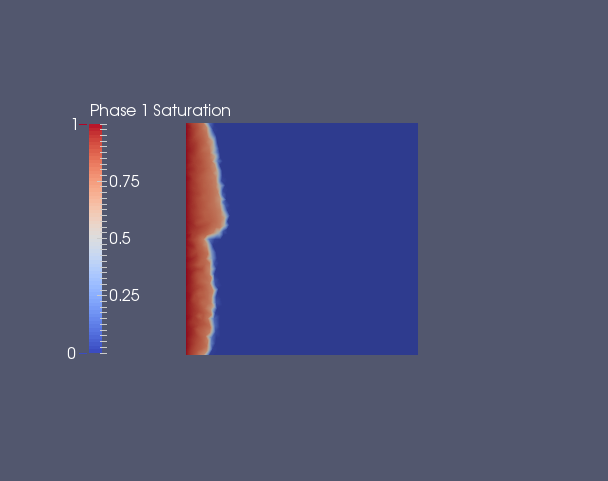
\includegraphics[width=.56\textwidth]{./Pics/BaseCase/BaseCase_Saturation_t_dot15.png}
      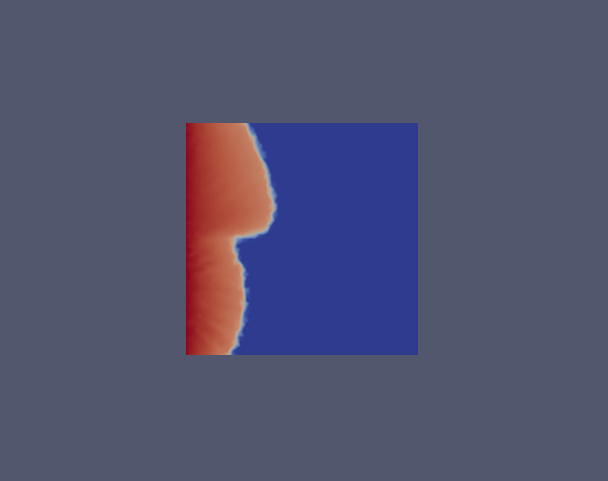
\includegraphics[width=.56\textwidth]{./Pics/BaseCase/BaseCase_Saturation_t_dot30.png}
      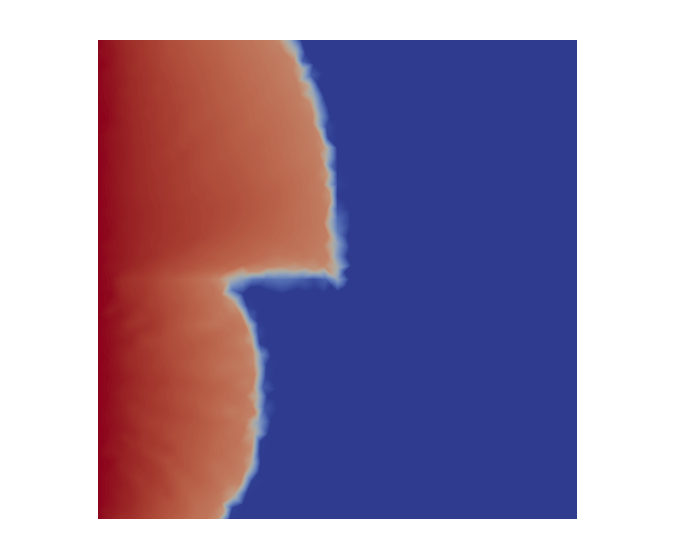
\includegraphics[width=.56\textwidth]{./Pics/BaseCase/BaseCase_Saturation_t_dot50.png}}
\vspace{0.cm}
\hbox{\hspace{0.5cm} (a) Phase 1 Saturation at t=0.15s \hspace{4.cm} (b) t=0.30s \hspace{3.75cm} (c) t=0.50s}
\vspace{0.5cm}
\hbox{
      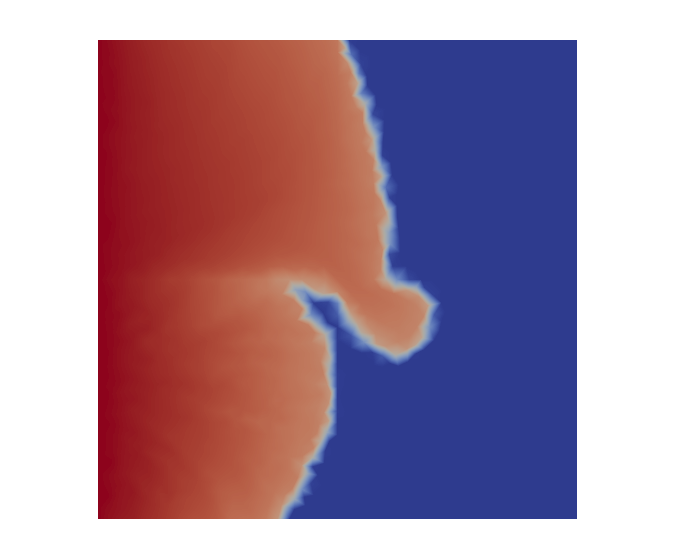
\includegraphics[width=.56\textwidth]{./Pics/BaseCase/BaseCase_Saturation_t_1dot15.png}
      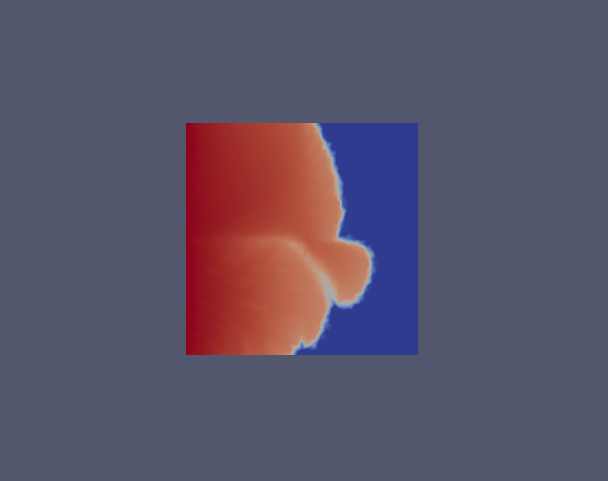
\includegraphics[width=.56\textwidth]{./Pics/BaseCase/BaseCase_Saturation_t_1dot75.png} 
      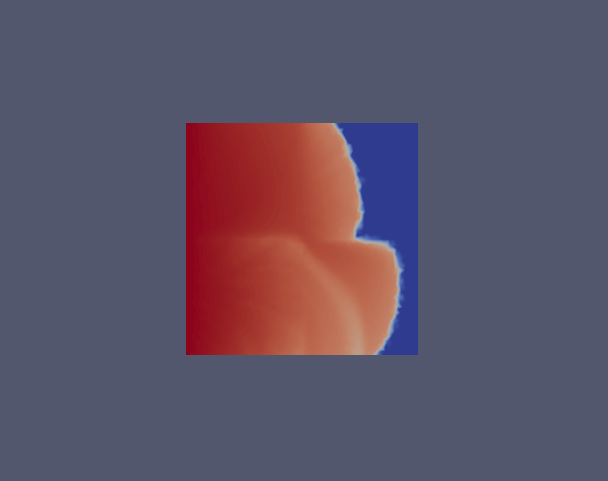
\includegraphics[width=.56\textwidth]{./Pics/BaseCase/BaseCase_Saturation_t_2dot95.png}}
\vspace{0.cm}
\hbox{ \hspace{1.cm} (d) t=1.15s \hspace{3.0cm} (e) t=1.75s   \hspace{4.0cm} (f) t=2.95s}
\vspace{0.cm}
}   
\caption{Simulated flow in a Hele-Shaw cell $\left(\text{{\it VR}=3, {\bf K}=10}^{-10}\text{cm}^{2}\right)$: (a) initial pressure profile $\left(\text{in g.cm}^{-1}\text{.s}^{-2}\right)$ with source and sink regions are explicitly shown along with dimensions (in cm); (b-f) snapshots of wetting phase saturation showing flow profile as the simulation evolves. The domain contains $26313$ \PN[1]{2} triangular elements.}
\label{fig:homoheleshaw_VN3}
\end{figure}
\end{landscape}
\clearpage
